\documentclass[useAMS,usenatbib]{mn2e}
%\documentclass[twocolumn]{emulateapj}
\usepackage{graphicx,natbib,color,multirow,amsmath}
\voffset=-0.8in

\definecolor{titlecol}{rgb}{0,0,1}
\definecolor{titlecol2}{rgb}{0,0.65,0}
\definecolor{titlecol3}{rgb}{0.99,0.4,0.}

%\definecolor{titledark}{rgb}{0,0,0.8}
%\definecolor{hilit}{rgb}{0,0,1}
%\definecolor{hilitdark}{rgb}{0,0,0.8}
%\font\sbf=cmssbx10 at 32.28pt %big font for headers

\font\nbf=cmssbx10 at 12.28pt %big font for headers

%%%%%%%%%%%%%%%%%%%%%%%%%%%%%%%
%%%% If you want to leave notes in the text feel free to define
%%%% your own colour above and a style below
%%%%%%%%%%%%%%%%%%%%%%%%%%%%%%%
\def\note		{\color{titlecol2} \nbf}
\def\noteb		{\color{titlecol} \nbf}
\def\notebsm	{\color{titlecol}}
\def\notec		{\color{titlecol2} \nbf}
\def\notecsm	{\color{titlecol2}}
\def\notek		{\color{titlecol3} }
\def\builderUC       {} % builder, unconfirmed

%%%%%%%%%%%%%%%%%%%%%%%%%%%%%%%
% For the eventual referee response
\def\changed    {\color{titlecol} }
%\def\changed    {}


%%%%%%%%%%%%%%%%%%%%%%%%%%%%%%%
%  Other stuff I use a lot
\def\oiii		{$\mathrm{\left[ O \textsc{iii}\right] }$}
\def\moiii		{\mathrm{\left[ O \textsc{iii}\right] }}
\def\nii		{$\mathrm{\left[ N \textsc{ii}\right] }$}
\def\mnii		{\mathrm{\left[ N \textsc{ii}\right] }}
\def\sii		{$\mathrm{\left[ S \textsc{ii}\right] }$}
\def\msii		{\mathrm{\left[ S \textsc{ii}\right] }}
\def\galfit     {{\tt GALFIT}}

\def\mmsun	{\rm{M}_{\odot}}
\def\fnobulge    {$f_{\rm no~bulge}$}
\def\mfnobulge {f_{\rm no~bulge}}
\def\fedgeon     {$f_{\rm edge-on}$}
\def\mfedgeon  {f_{\rm edge-on}}
\def\fcnobulge    {$f_{\rm confirmed~no~bulge}$}
\def\mfcnobulge {f_{\rm confirmed~no~bulge}}


%\def\lesssim{\mathrel{\hbox{\rlap{\hbox{\lower5pt\hbox{$\sim$}}}\hbox{$<$}}}}
%\def\gtrsim{\mathrel{\hbox{\rlap{\hbox{\lower5pt\hbox{$\sim$}}}\hbox{$>$}}}}
%new defs of lesssim gtrsim that I think look better
\def\lesssim{\mathrel{\hbox{\rlap{\hbox{\lower3pt\hbox{$\sim$}}}\hbox{\raise2pt\hbox{$<$}}}}}
\def\gtrsim{\mathrel{\hbox{\rlap{\hbox{\lower3pt\hbox{$\sim$}}}\hbox{\raise2pt\hbox{$>$}}}}}


\newcommand\nodata{ ~$\cdots$~ }




\begin{document}

\title[Galaxy Zoo: CANDELS Data Release]{Galaxy Zoo: Detailed Morphological Classifications for 48,000 galaxies from CANDELS\thanks{This publication has been made possible by the participation of more than {\notebsm COUNT} volunteers in the Galaxy Zoo project. Their contributions are
individually acknowledged at http://authors.galaxyzoo.org/ .} } 

\author[Simmons et al.]{\parbox[t]{16cm}{B. D. Simmons$^{1}\thanks{E-mail: brooke.simmons@astro.ox.ac.uk}$, {\notebsm and a \emph{lot} of other people to be named later}
%Chris Lintott$^{1,3}$, 
%Kyle W. Willett$^{5}$, 
%Karen L. Masters$^{2,4}$, 
%Robert C. Nichol$^{2,4}$, 
%William C. Keel$^{6}$, 
%Thomas Melvin$^{2}$, 
%R. J. Smethurst$^{1}$, 
%Edmond Cheung$^{7}$, 
%Kevin Schawinski$^{8}$, 
%Michael Rutkowski$^{5}$,
%Jeyhan S. Kartaltepe$^{9,}$\footnote{Hubble Fellow}, 
%Kevin R. V. Casteels$^{11}$, 
%Christopher J. Conselice$^{12}$,
%Omar Almaini$^{12}$, 
%Henry C. Ferguson$^{13}$,
%Lucy Fortson$^{5}$, 
%William Hartley$^{12,8}$, 
%Dale Kocevski$^{14}$,
%Anton M. Koekemoer$^{13}$,
%Daniel H. McIntosh$^{15}$,
%Alice Mortlock$^{12}$, 
%{\builderUC Jeffrey A. Newman$^{16}$,}
%Jamie Ownsworth$^{12}$, 
%Steven Bamford$^{12}$,
%{\builderUC Tomas Dahlen$^{13}$,} 
%{\builderUC Sandra M. Faber$^{17}$,}
%{\builderUC Steven L. Finkelstein$^{18}$,} 
%{\builderUC Adriano Fontana$^{19}$,}
%{\builderUC Audrey Galametz$^{19}$,}
%N. A. Grogin$^{13}$,
%{\builderUC Ruth Gr\"utzbauch$^{12, 20}$,} 
%{\builderUC Yicheng Guo$^{17}$,}
%{\builderUC Boris H\"au\ss ler$^{12,21,1}$,}
%Kian Jek$^{22}$,
%Sugata Kaviraj$^{21}$,
%Ray A. Lucas$^{13}$,
%{\builderUC Michael Peth$^{23}$,}
%{\builderUC Mara Salvato$^{24}$,} 
%{\builderUC Tommy Wiklind$^{25}$,} 
%{\builderUC Stijn Wuyts$^{24}$}
%
\vspace{0.1in} }\\
$^{1}$Oxford Astrophysics, Denys Wilkinson Building, Keble Road, Oxford OX1 3RH, UK\\
%$^{2}$Institute of Cosmology \& Gravitation, University of Portsmouth, Dennis Sciama Building, Portsmouth PO1 3FX, UK\\
%$^{3}$Adler Planetarium, 1300 S. Lake Shore Drive, Chicago, IL 60605, USA\\
%$^{4}$SEPnet,\thanks{www.sepnet.ac.uk} South East Physics Network\\
%$^{5}$School of Physics and Astronomy, University of Minnesota, 116 Church St. SE, Minneapolis, MN 55455, USA\\
%$^{6}$Department of Physics and Astronomy, University of Alabama, Box 870324, Tuscaloosa, AL 35487, USA\\
%$^{7}$Department of Astronomy and Astrophysics, 1156 High Street, University of California, Santa Cruz, CA 95064, USA\\
%$^{8}$Institute for Astronomy, ETH Z\"urich, Wolfgang-Pauli-Strasse 27, CH-8093 Z\"urich, Switzerland\\
%$^{9}$National Optical Astronomy Observatory, 950 N. Cherry Ave., Tucson, AZ, 85719, USA\\
%$^{10}$Department of Astronomy, University of Michigan, Ann Arbor, MI 48104, USA\\
%$^{11}$Institut de Cincies del Cosmos. Universitat de Barcelona (UB-IEEC), Mart i Franqus 1, E-08028 Barcelona, Spain\\
%$^{12}$School of Physics \& Astronomy, University of Nottingham, Nottingham NG7 2RD\\
%$^{13}$Space Telescope Science Institute, 3700 San Martin Drive, Baltimore, MD 21218\\
%$^{14}$Department of Physics and Astronomy, University of Kentucky, Lexington, KY 40506, USA\\
%$^{15}$Department of Physics, University of Missouri-Kansas City, 5110 Rockhill Road, Kansas City, MO 64110, USA\\
%$^{16}$Department of Physics and Astronomy \& PITT PACC, University of Pittsburgh, Pittsburgh, PA 15217, USA\\
%$^{17}$UC Observatories/Lick Observatory and Department of Astronomy and Astrophysics, University of California, Santa Cruz, CA 95064, USA\\
%$^{18}$Department of Astronomy, The University of Texas at Austin, Austin, TX 78712, USA\\
%$^{19}$INAF-Osservatorio Astronomico di Roma, Via Frascati 33, I-00040, Monteporzio, Italy\\
%$^{20}$Centre for Astronomy and Astrophysics, University of Lisbon, P-1349-018 Lisbon, Portugal\\
%$^{21}$Centre for Astrophysics Research, University of Hertfordshire, College Lane, Hatfield AL10 9AB, UK\\
%$^{22}$Galaxy Zoo Volunteer\\
%$^{23}$Department of Physics and Astronomy, The Johns Hopkins University, Baltimore, MD 21218, USA\\
%$^{24}$Max-Planck-Institut f{\"u}r extraterrestrische Physik, Giessenbachstrasse 1, D�85748 Garching bei M{\"u}nchen, Germany\\
%$^{25}$European Southern Observatory/Joint ALMA Observatory, 3107 Alonso de Cordova, Santiago, Chile\\
   }

\maketitle
  
\label{firstpage}
  
%\clearpage

\begin{abstract}

{\notebsm To be rewritten, probably last.}

Galaxies are sometimes really far away. The distant ones are pretty cool, because they tell us what the Universe was like back when it was just a kid, or maybe a teenager. You really have to look hard to see these galaxies, but once you do, what you do see tells you a whole lot. I mean, it's not exactly a WYSIWYG type of thing: there's a lot of work to figure out what the faint stuff you see really means. We did a bunch of work, and we think we did pretty well. Also, we compared to others who have done different kinds of work to try and answer some of the same questions. But we have a unique way of answering them, so here are those answers, and you can use them to answer other questions about the Universe.


  \end{abstract}
  
  \begin{keywords}
  
  galaxies: general 
  --- 
  galaxies: evolution
  --- 
  galaxies: morphology %not actually a keyword 
  --- 
  galaxies: structure
  
  \end{keywords}

%%%%%%%%%%%%%%%%%%%%%%%%%%%%%%%%%%%%%%%%%%%%%%
%
%  
\section{Introduction}
%
%
%%%%%%%%%%%%%%%%%%%%%%%%%%%%%%%%%%%%%%%%%%%%%%

{\notebsm Outline:}\\
Galaxy morphologies trace physics \& dynamics and are therefore important.

They have a long history and there are many types, including those that use proxies [which are useful but not without problems] and those that reduce a galaxy and its billions of stars to a single number [same]. Visual morphologies are in many ways still ideal as they are able to provide incredibly detailed information about galaxies.

Visual morphologies have a scale problem without many eyes, and they're often not quantified. Galaxy Zoo to the rescue.

Galaxy Zoo started in 2007 and has provided robust, quantified visual classifications for more than 1,000,000 galaxies to $z \sim 1$. 

Much use has been made of these, including [summarize and include non-GZ papers].

Here we present the visual morphologies of galaxies imaged by the $HST$ treasury survey CANDELS.

Section summary and cosmology.




%%%%%%%%%%%%%%%%%%%%%%%%%%%%%%%%%%%%%%%%%%%%%%
%
%
\section{Observational Data}\label{sec:data}
%
%
%%%%%%%%%%%%%%%%%%%%%%%%%%%%%%%%%%%%%%%%%%%%%%

\subsection{Images}\label{sec:images}

% Note this is lifted directly from the bar paper so I should probably mix it up a bit later
The Cosmic Assembly Near-infrared Extragalactic Legacy Survey \citep[CANDELS;][]{grogin11,koekemoer11} is an \emph{HST} Treasury programme combining optical and near-infrared imaging from the Advanced Camera for Surveys (ACS) and Wide Field Camera 3 (infrared channel; WFC3/IR) across five well-studied survey fields {(GOODS-North and -South, \citeauthor{giavalisco04} \citeyear{giavalisco04}; EGS, \citeauthor{davis07} \citeyear{davis07}; UDS, \citeauthor{lawrence07} \citeyear{lawrence07}, \citeauthor{cirasuolo07} \citeyear{cirasuolo07}; and COSMOS, \citeauthor{scoville07} \citeyear{scoville07}) using a two-tiered ``deep'' and ``wide'' approach. Each of the wide fields (UDS, COSMOS, EGS and flanking fields to the GOODS-S and GOODS-N deep fields) are imaged over 2 orbits in WFC3/IR, split in a 2:1 ratio between filters F160W and F125W, respectively, with parallel exposures in F606W and F814W using ACS. Each of the deep fields (GOODS-S and GOODS-N) are imaged over at least 4 orbits each in both the F160W and F125W filters and 3 orbits in the F105W filter, with ACS exposures in F606W and F814W in parallel. These are reduced and combined to produce a single mosaic for each field in each band, with drizzled resolutions of $0.03^{\prime\prime}$ and $0.06^{\prime\prime}$ per pixel for ACS and WFC3/IR, respectively \citep[a process described in detail by][]{koekemoer11}.

Here we use the CANDELS ACS and WFC3/IR images from within the first set of data to be classified within the Galaxy Zoo interface. Those data cover the COSMOS, GOODS-South, and UDS fields. The 4th release of Galaxy Zoo included all detections with $H \leq 25.5$ from these 3 combined fields, comprising 49,555 unique images. These were shown to visitors to the website galaxyzoo.org{\footnote{Archived at zoo4.galaxyzoo.org}} starting on the 10th of September, 2012.  

The images shown to the public are colour composites of ACS $I$ ($F814W$), WFC3 $J$ ($F125W$), and WFC3 $H$ ($F160W$) filters for the blue, green and red channels, respectively. The angular sizes of the images in different filters are matched, and the native point-spread functions (PSFs) are used. The images are combined with an asinh stretch \citep[described in detail in][]{luptonasinh} with a non-linearity value of {\notebsm 3.0}. 

Sources in the dataset vary greatly in size and surface brightness, and therefore a single set of values for channel scalings is not adequate to capture the variety of features across the images. We therefore use a variable scaling based on the {\notebsm magnitude and size} of each target source. For each image the R, G, and B channels have a fixed ratio of {\notebsm [not sure; must get this from Jeyhan]}, and the multiplier can vary between {\notebsm A and B}. Figure \ref{fig:imageexamples} shows examples of these colour composites across a wide range of source fluxes and sizes. 

Each colour image is 424 pixels square. The angular size of the image varies, such that the colour image encompasses at least {\notebsm 3 times the 80\% flux radius of the target source}, with a minimum screen-to-WFC3 zoom ratio of {\notebsm 1:10} and a maximum ratio of {\notebsm 3:1}. The Galaxy Zoo interface loads the normal colour images by default, and the user may choose to display an inverted colour image, but may not otherwise change the image scaling or size within the software while performing the classification.



\subsection{Photometry}

Brief description of photometric catalogs. Focus on $IJH$ because that's all the images consider. Do mention all the extra stuff available, but note that the classifications themselves don't depend on them.
%The debiasing will, though, because the photometric redshifts do.



\subsection{Redshifts}\label{sec:z}

Some of them have speczs. Lots of them have photzs, including CANDELS, 3D-HST and several previous surveys.
%I'm thinking the first thing to do is pick a redshift for all the sources, and settle on it, before any other analysis proceeds.
%Also it would be helpful to match each ID we use to the CANDELS unique ID that the team uses. Even if we don't publish it.

Comparison of photozs and speczs; might be able to just reference the other papers.

What do we do about those without redshifts? We use them with caution, I guess.



\subsection{Simulated Images}\label{sec:ferengi}

Describe simulations and what we'll use them for.




%%%%% [FIGURE: Bar fractions and mags of sample] %%%%%
%\begin{figure*}
%\includegraphics[scale=0.273]{tree_part_with_selection.eps}
%\caption{
%\emph{Left:} Partial Galaxy Zoo: CANDELS classification tree, starting with the first question (top) and leading to the bar feature question. There are 17 questions total in the tree; the bar question is a 4th-tier task. \emph{Right:} Selection of the featured, not-edge-on disk galaxy sample (876 galaxies) in GZ-CANDELS; relative box areas are scaled to the sample sizes. This selection was made independently of restrictions on redshift or luminosity (a full description of the sample selection is given in Section \ref{sec:sample}). Eight independent classifiers subsequently examined each of the 876 disk galaxies for evidence of a bar. 
%}
%\label{fig:sampleselection}
%\end{figure*}
%%%%% END FIGURE %%%%%




%%%%% [FIGURE: Example images] %%%%%
%\begin{figure*}
%\includegraphics[scale=1.0]{barfig_3.eps}
%\caption{
%Examples of disk galaxies in GZ-CANDELS whose bar vote percentage $(p_{bar})$ places them in the unbarred (top row) and barred (bottom row) sub-samples.
%}
%\label{fig:gals}
%\end{figure*}
%%%%% END FIGURE %%%%%




%%%%%%%%%%%%%%%%%%%%%%%%%%%%%%%%%%%%%%%%%%%%%%
%
%
\section{Classification Data}\label{sec:classifications}
%
%
%%%%%%%%%%%%%%%%%%%%%%%%%%%%%%%%%%%%%%%%%%%%%%

\subsection{Decision Tree}

%%%%% [FIGURE: Example images] %%%%%
\begin{figure*}
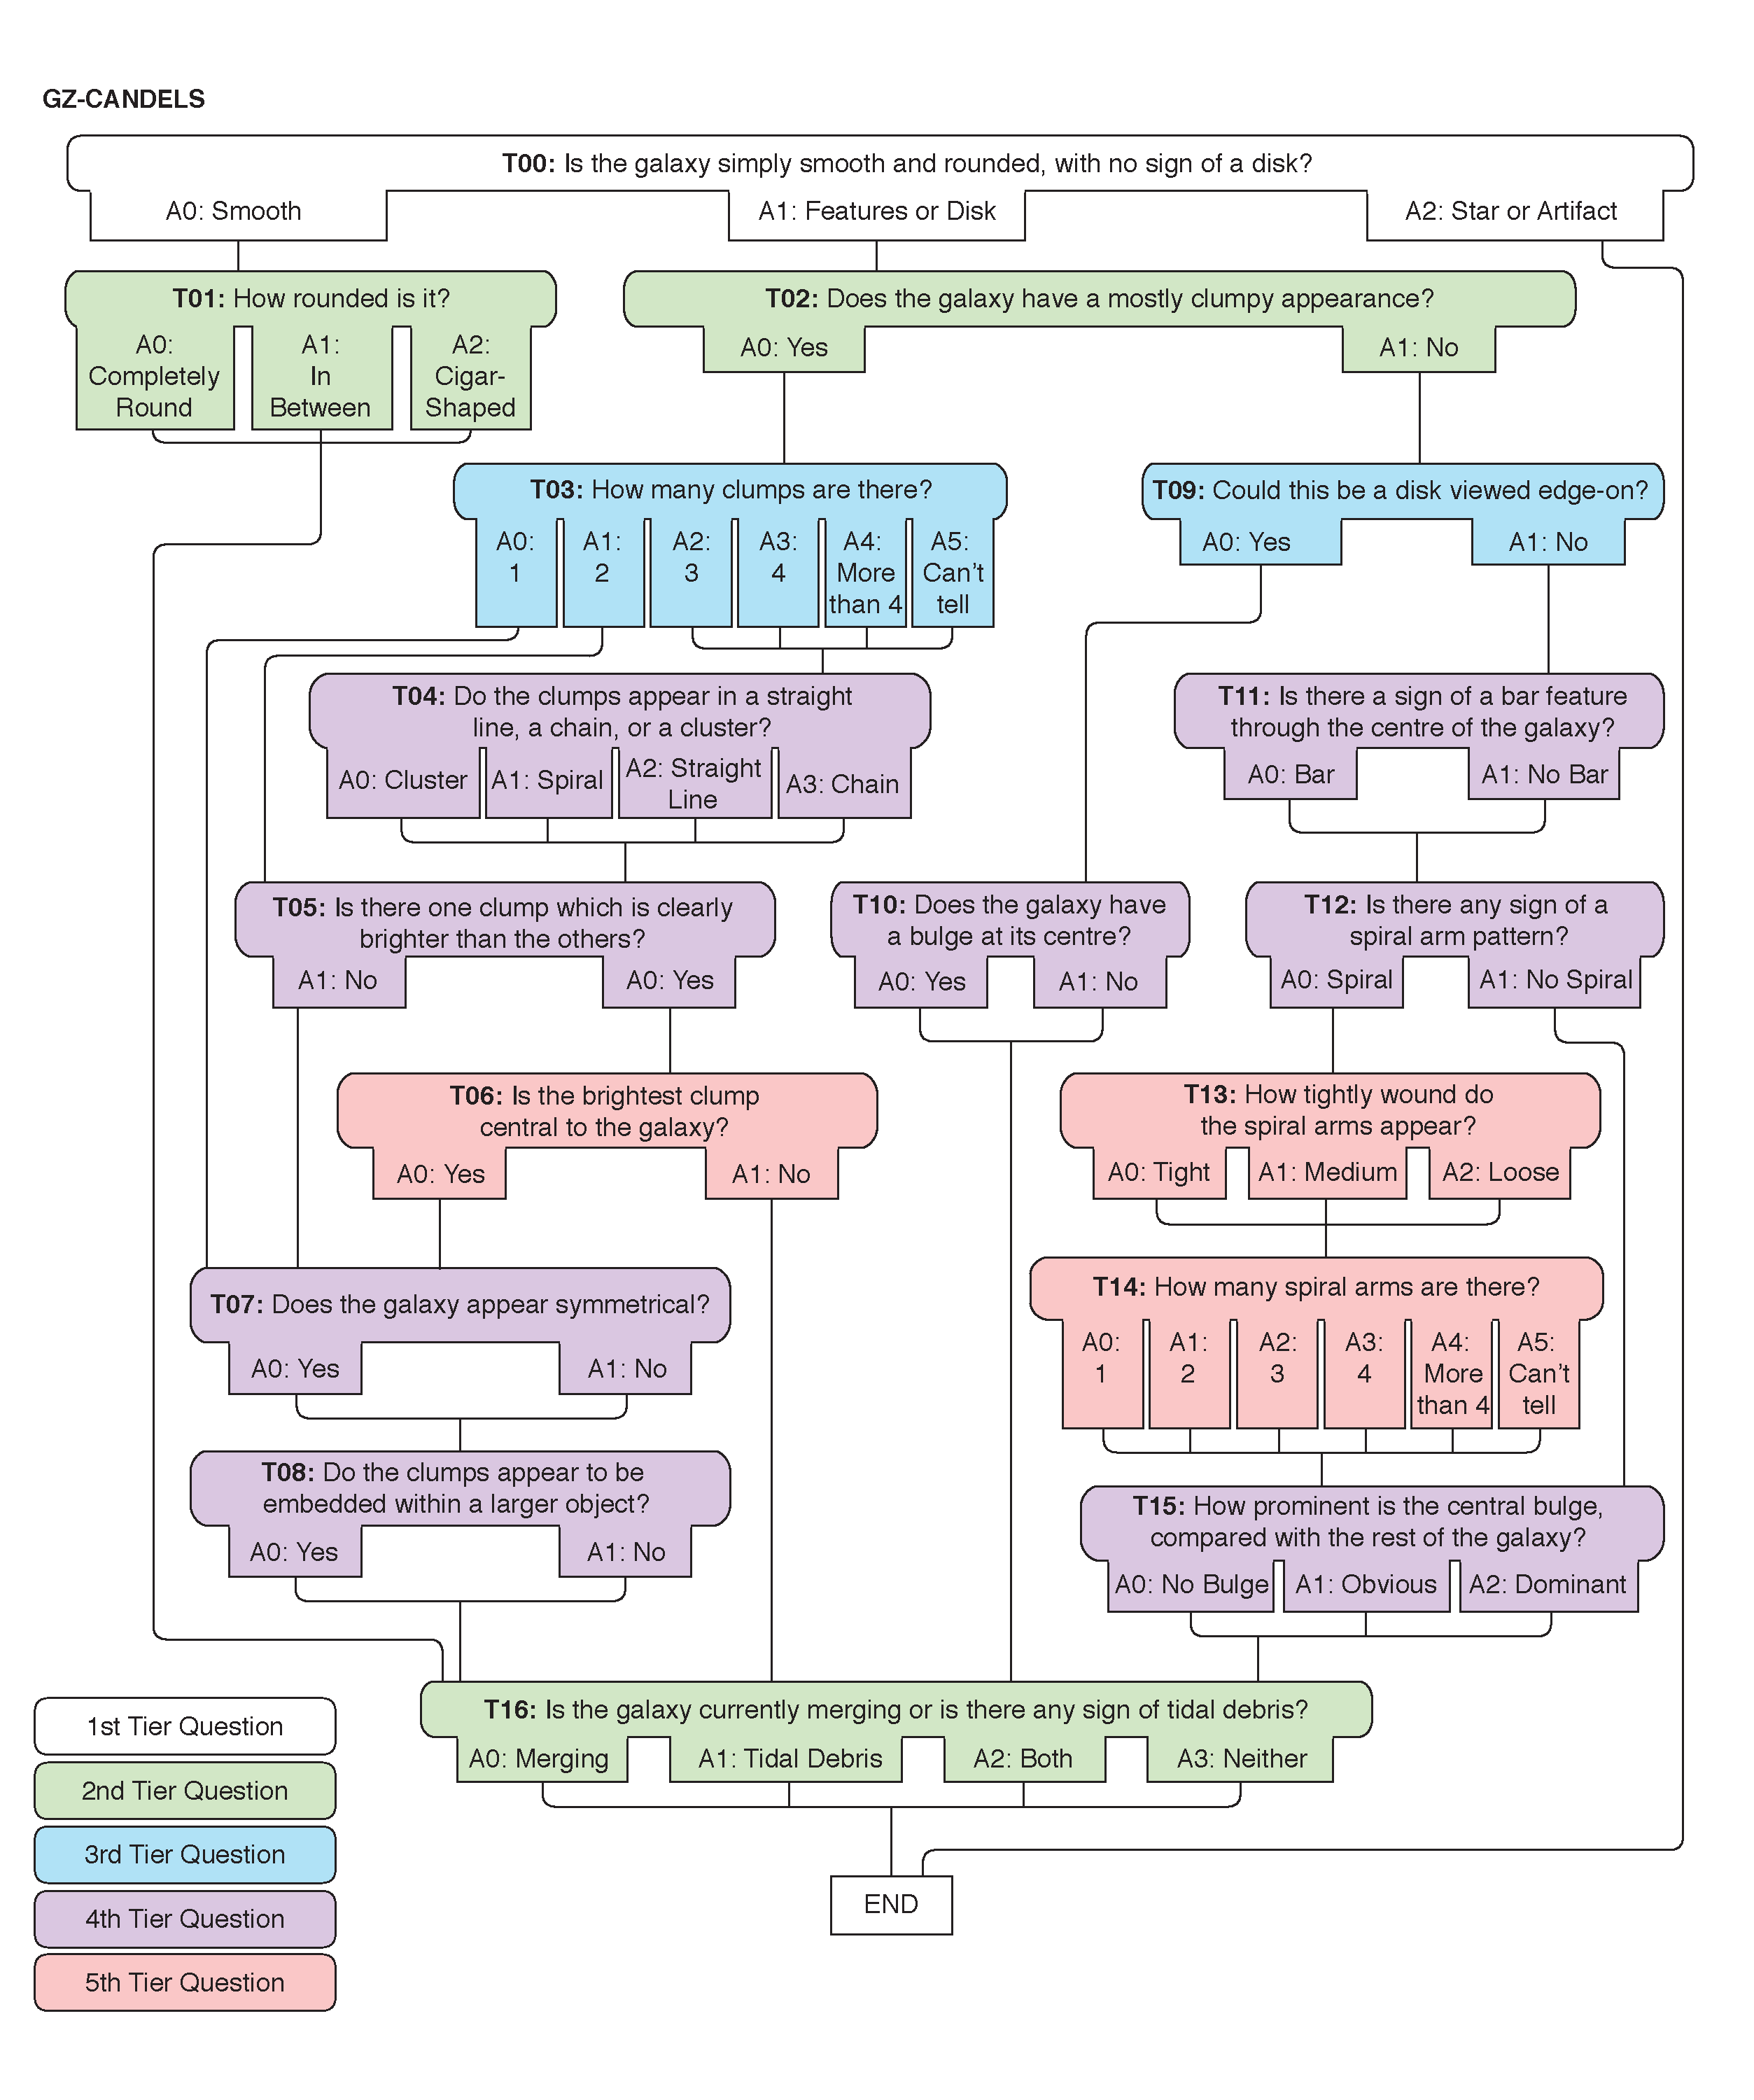
\includegraphics[scale=0.45]{candels_classification_tree_withlabels_new.eps}
\caption{
The Decision Tree for Galaxy Zoo: CANDELS
}
\label{fig:tree}
\end{figure*}
%%%%% END FIGURE %%%%%

Details on the decision tree, plus a table mapping questions and answers to unique tasks and answers, like the one in Willett et al. 2013.



\subsection{Raw classifications}

Basic details on raw classifications, including the start and end dates considered in this paper, how many classifications which galaxies have, why some have less than others and some more. 

How many users participated, and the distribution of classifications (typical number per person, number signed in and not, maybe that square diagram Old Weather uses). 



\subsection{User Weighting}

Note: we may discuss other weighting if that proves useful.

\subsubsection{Consensus Weighting}

\subsubsection{IBCC}



%%%%%%%%%%%%%%%%%%%%%%%%%%%%%%%%%%%%%%%%%%%%%%
%
%  
\section{Comparison to other classifications}
%
%
%%%%%%%%%%%%%%%%%%%%%%%%%%%%%%%%%%%%%%%%%%%%%%

  
Kartaltepe et al. 2014

CAS? Gini? M20?



%%%%%%%%%%%%%%%%%%%%%%%%%%%%%%%%%%%%%%%%%%%%%%
%
%  
\section{Some kind of initial result}
%
%
%%%%%%%%%%%%%%%%%%%%%%%%%%%%%%%%%%%%%%%%%%%%%%

Hubble Sequence, maybe?




%%%%%%%%%%%%%%%%%%%%%%%%%%%%%%%%%%%%%%%%%%%%%%
%
%  
\section{Summary}
%
%
%%%%%%%%%%%%%%%%%%%%%%%%%%%%%%%%%%%%%%%%%%%%%%

Galaxies! We have so many galaxies!

  
%%%%%%%%%%%%%%%%%%%%%%%%%%%%%%%%%%%%%%%%%%%%%%
%%%%%%%%%%%%%%%%%%%%%%%%%%%%%%%%%%%%%%%%%%%%%%
%%%%%%%%%%%%%%%%%%%%%%%%%%%%%%%%%%%%%%%%%%%%%%
%%%%%%%%%%%%%%%%%%%%%%%%%%%%%%%%%%%%%%%%%%%%%%
%
%
\section*{Acknowledgments}
%
%
%%%%%%%%%%%%%%%%%%%%%%%%%%%%%%%%%%%%%%%%%%%%%%

%TOPCAT \citep{taylor05} and an OS X widget form of the JavaScript Cosmology Calculator \citep{wright06} were used while preparing this paper. 
%
%BDS gratefully acknowledges support from the Oxford Martin School, Worcester College and Balliol College, Oxford.
%
%TM acknowledges funding from the Science and Technology Facilities Council ST/J500665/1.
%
%KLM acknowledges funding from The Leverhulme Trust as a 2010 Early Career Fellow.
%
%KWW and LF acknowledge funding from the UMN Grant-In-Aid program. 
%
%RCN acknowledges STFC Rolling Grant ST/I001204/1 to ICG for �Survey Cosmology and Astrophysics�. 
%
%KS gratefully acknowledges support from Swiss National Science Foundation Grant PP00P2\_138979/1. 
%

The development of Galaxy Zoo was supported in part by the Alfred P. Sloan Foundation. Galaxy Zoo was supported by The Leverhulme Trust. 

This work is based on observations taken by the CANDELS Multi-Cycle Treasury Program with the NASA/ESA HST, which is operated by the Association of Universities for Research in Astronomy, Inc., under NASA contract NAS5-26555.
  
\bibliographystyle{mn2e}
\bibliography{refs}  


  
\end{document}
  
